\documentclass[12pt]{article}

\usepackage[english]{babel}
\usepackage[utf8]{inputenc}
\usepackage{xspace}
\usepackage{amsmath,amssymb,amsfonts,mathrsfs,latexsym,stmaryrd}
\usepackage{mathtools}
\usepackage{amsthm}
\usepackage{stackrel}
\usepackage{xcolor}
\usepackage{widetable}
\usepackage{graphicx}
\usepackage{tikz}
\usetikzlibrary{automata,positioning}

\newcommand{\A}{\ensuremath{\mathcal{A}}\xspace}
\newcommand{\Buchi}{\ensuremath{\mathcal{A} = (\mathcal{Q},A,\Delta,q_0,F)}\xspace}
\newcommand{\congAlpha}{\ensuremath{\cong_\alpha}\xspace}
\newcommand{\congAlphaM}{\ensuremath{\congAlpha^m}\xspace}
\newcommand{\buchi}{B\"uchi }

\title{Automatic System Verification\\Exercices}
\author{
        Cominato Enrico 137396 \\
                Department of Computer Science\\
        Univeristy of Udine
}
\date{\today}



\begin{document}
\maketitle

\section{Exercices on the automata's notes}
\subsection*{Esercizio 2.3}
\textit{Sia $\A$ l'automa dell'Esempio 2.2. Si consideri l'automa $\A'$ ottenuto da $\A$ rimuovendo lo stato $q_0$, e le transizioni in esso entranti e da esso uscenti, e facendo diventare $q_1$ il nuovo stato iniziale. Si stabilisca se $\A$ e $\A'$ riconoscono o meno lo stesso linguaggio} \\
\tikzset{every picture/.style={line width=0.75pt}} %set default line width to 0.75pt        
Riporto di seguito i due grafi.
\begin{center}
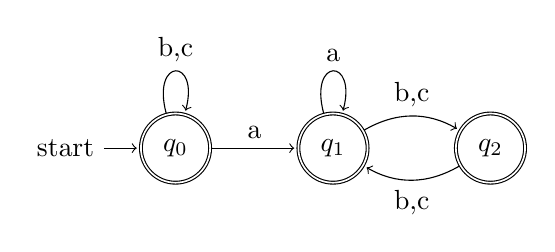
\begin{tikzpicture}[shorten >=1pt,node distance=2cm,on grid,auto] 
	\node[state,initial,accepting] (q_0)   {$q_0$}; 
   	\node[state,accepting] (q_1) [right=of q_0]  {$q_1$};  
   	\node[state,accepting] (q_2) [right=of q_1] {$q_2$};
    \path[->] 
    (q_0) edge [loop above] node {b,c} (q_0)
          edge  node {a} (q_1)
    (q_1) edge [loop above] node {a} (q_1)
          edge [bend left] node {b,c} (q_2)
    (q_2) edge [bend left] node  {b,c} (q_1);
\end{tikzpicture}
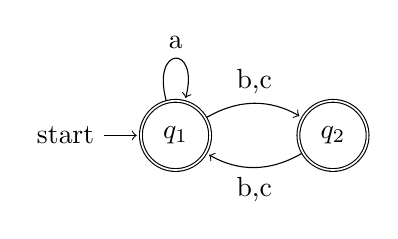
\begin{tikzpicture}[shorten >=1pt,node distance=2cm,on grid,auto] 
   \node[state,initial,accepting] (q_1)   {$q_1$};  
   \node[state,accepting] (q_2) [right=of q_1] {$q_2$};
    \path[->] 
    (q_1) edge [loop above] node {a} (q_1)
          edge [bend left] node {b,c} (q_2)
    (q_2) edge [bend left] node  {b,c} (q_1);
\end{tikzpicture}
\end{center}

I due linguaggi non sono uguali. Per esempio la $\omega -parola$ $babcabca...$ appartiene al primo dei due automi, ma non al secondo (da $q_1$ andiamo in $q_2$ ma da li possiamo leggere solo una b oppure una c)


\subsection*{Esercizio 2.4}
\textit{Si costruisca l'automa $\A'$ che riconosce la variante finita (linguaggio di parole finite) dell'Esempio 2.2}\\
Il linguaggio richiesto è il seguente:\\
\textit{L'insieme delle parole finite su $A=\{a,b,c\}$ tali che tra ogni
coppia di occorrenze consecutive di a esiste un numero pari di occorrenze di simboli diversi da a.}\\
Osservazione: una parola con una sola occorrenza di $a$ deve essere sempre accettata.\\
L'automa risultante quindi è lo stesso dell'esempio 2.2, solo che le run su questo automa sono finite.
% Esempio regex ^[bc]*(a([bc][bc])*)*[bc]?$
% per completare l'automa in modo che legga tutte le possibili parole basta aggiungere uno stato q_3 non terminale raggiungibile da q_2 con "a" e su cui si cicla all'infinito con {a,b,c}
\begin{center}
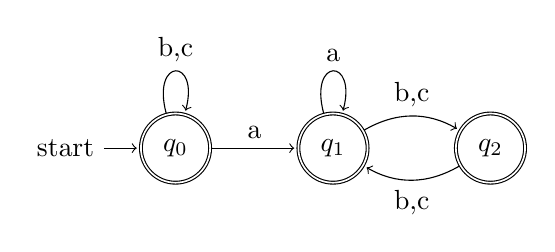
\begin{tikzpicture}[shorten >=1pt,node distance=2cm,on grid,auto] 
	\node[state,initial,accepting] (q_0)   {$q_0$}; 
   	\node[state,accepting] (q_1) [right=of q_0]  {$q_1$};  
   	\node[state,accepting] (q_2) [right=of q_1] {$q_2$};
    \path[->] 
    (q_0) edge [loop above] node {b,c} (q_0)
          edge  node {a} (q_1)
    (q_1) edge [loop above] node {a} (q_1)
          edge [bend left] node {b,c} (q_2)
    (q_2) edge [bend left] node  {b,c} (q_1);
\end{tikzpicture}
\end{center}


\subsection*{Esercizio 2.5}
\textit{Sia W il linguaggio riconosciuto dall'automa \A' dell'Esercizio 2.4. Si caratterizzi il linguaggio $\overrightarrow{W}$.}

Riprendo la definizione di $\overrightarrow{W}$: 
$$\overrightarrow{W}=\{\alpha\in A^\omega \; t.c.\; \exists^\omega n \; \alpha(0,n) \in W\}$$
Sono quindi tutte quelle $\omega$-parole di cui ogni prefisso finito appartiene a $W$.
Analizziamo per casi:
\begin{itemize}
	\item la parola non ha neppure una $a$: in questo caso ogni suo prefisso appartiene a $W$ perchè le parole $(b|c),(b|c)^2,(b|c)^3,\ldots,(b|c)^n,\ldots \in W$
	\item la parola ha una sola occorrenza di $a$: anche in questo caso ogni suo prefisso appartiene a $W$ perchè:
	\begin{itemize}
		\item come visto nel punto precedente, fino a che non si incontra la lettera $a$ le parole appartengono a $W$
		\item dopo l'occorrenza di $a$, ancora tutti i prefissi appartengono a $W$, dato che tutte le parole finite con una sola occorrenza di $a$ appartengono a $W$
	\end{itemize}	
	\item infine tutti gli altri casi sono parole con un più di una occorrenza di $a$: dove abbiamo che ogni prefisso, o ricade in uno dei precedenti casi, oppure è una parola che tra ogni
coppia di occorrenze consecutive di a esiste un numero pari di occorrenze di simboli diversi da a e che quindi appartiene a $W$.
\end{itemize}

In questo caso abbiamo che $W^\omega = \overrightarrow{W}$.


\subsection*{Esercizio 2.7}
\paragraph*{Teorema 2.6}
\begin{enumerate}
	\item Se $V \subseteq A^*$ è regolare, allora $V^\omega$ è $\omega -regolare$
	\item Se $V \subseteq A^*$ è regolare e $L \subseteq A^\omega$ è $\omega -regolare$, allora $V\cdot L$ è $\omega -regolare$
	\item Se $L_1, L_2\subseteq A^*$ sono $\omega -regolari$, allora $L_1 \cup L_2$ e $L_1 \cap L_2$sono $\omega -regolari$
\end{enumerate}
\textit{Dimostrare le proprietà (2) e (3) del teorema}

Dimostro \textit{(2)}. Siano $\mathcal{A}, \mathcal{B}$ automi tali che $\mathcal{A}$ accetta V e $\mathcal{B}$ accetta L, allora possiamo costruire $\mathcal{C}$ unendo tutti gli stati finali di $\mathcal{A}$ con lo stato iniziale di $\mathcal{B}$. Otteniamo così un'automa che legge il linguaggio $V\cdot L$, quindi $V \cdot L$ è $\omega$-regolare.

Dimostro \textit{(3)}. Per quanto riguarda l'unione, prendiamo $\mathcal{A}, \mathcal{B}$ automi tali che $\mathcal{A}$ accetta $L_1$ e $\mathcal{B}$ accetta $L_2$. Costruiamo $\mathcal{C}$ unendo gli stati iniziali di $\mathcal{A}$ e $\mathcal{B}$. Abbiamo quindi che $\mathcal{C}$ accetta tutte le parole di $L_1 \cup L_2$. Sappiamo inoltre che i linguaggi $\omega$-regolari sono chiusi per complementazione, quindi possiamo riscrivere $L_1 \cap L_2 = \neg (\neg L_1 \cup \neg L_2)$ ed ottenere la chiusura per intersezione.

\subsection*{Esercizio 2.13}
\textit{Fornire un esempio di parola non definitivamente periodica}

Un esempio è: $$ ababbab^3ab^4ab^5...$$


\subsection*{Esercizio 2.16}
\textit{Dimostrare che una congruenza è una relazione di equivalenza invariante destra}

Invariante a destra significa che $\forall x,y,z \in A$, se $x \sim y$ allora $xz \sim yz$. Questo è sempre vero perchè, concatenando la stessa parola ad $x,y$ finiremo in un'unica classe di equivalenza.

\subsection*{Esercizio 2.19}
\textit{Dato un automa di \buchi $\Buchi$, dimostrare che, per ogni $s,s' \in \mathcal{Q}$, $W^F_{ss'}$ è regolare}

Un linguaggio è regolare se esiste un'automa in grado di accettarlo. Per poterlo accettare deve avere almeno uno stato finale. Quindi se eliminiamo dall'automa \A, tutti gli stati e le relazioni non interessate dai possibili cammini tra $s$ e $s'$ otteniamo un automa in grado di leggere solo $W^F_{ss'}$, e questo fa di lui un linguaggio regolare.

\subsection*{Esercizio 2.23}
\textit{Dimostrare che la relazione $\approx_A$ è una congruenza di indice finito}

Perchè $\approx_A$ sia una congruenza deve valere che $\forall u,u',v,v' \in A^*$ se $ u\approx_A v$ e $u' \approx_A v'$ allora $uu' \approx_A vv'$. Questo è vero perchè avendo $ u \approx_A v$ e $u' \approx_A v'$, allora $\exists t$ tale che:
\begin{itemize}
	\item $s \rightarrow_u t \Leftrightarrow s \rightarrow_v t$
	\item $s \rightarrow_u^F t \Leftrightarrow s \rightarrow_v^F t$
	\item $t \rightarrow_{u'} s' \Leftrightarrow t \rightarrow_{v'} s'$
	\item $t \rightarrow_{u'}^F s' \Leftrightarrow t \rightarrow_{v'}^F s'$
\end{itemize} 
Quindi abbiamo che $\forall s,s' \in Q$:
\begin{itemize}
	\item $s \rightarrow_{uu'} s' \Leftrightarrow s \rightarrow_{vv'} s'$
	\item $s \rightarrow_{uu'}^F s' \Leftrightarrow s \rightarrow_{vv'}^F s'$
\end{itemize} 
e quindi $uu' \approx_A vv'$.
Il resto della dimostrazione è già stata svolta negli appunti.

\subsection*{Esercizio 2.25}
\textit{Si dimostri che la relazione $\congAlpha$ è una relazione di equivalenza sui naturali di indice finito}

Riprendo la definizione di $\congAlpha$. Sia $\sim$ una congruenza su $A^*$ di indice finito. Sia $\alpha \in A^\omega$ e siano $k,k'$ posizioni. Diciamo che 
$k\congAlphaM k'$ ($k,k'$ si riuniscono in $m>k,k'$) se $\alpha(k,m)\sim\alpha(k',m)$. Diciamo che $k\congAlpha k'$ se esiste $m$ per cui $k \congAlphaM k'$.

Dimostro che è una relazione di equivalenza:
\begin{itemize}
	\item \textbf{Riflessività}: $\forall k \in \mathbb{N}$ è sempre vero che $k\congAlpha k$ perchè $k\congAlpha k \Leftrightarrow \exists m\;t.c.\;\alpha(k,m)\sim\alpha(k,m)$ e questo è vero $\forall k$ perchè $\sim$ è una relazione di equivalenza
	\item \textbf{Simmetria}: $\forall k,k' \in \mathbb{N}$ è sempre vero che $k\congAlpha k' \Rightarrow k' \congAlpha k$ perchè $k\congAlpha k' \Leftrightarrow \exists m\;t.c.\;\alpha(k,m)\sim\alpha(k',m)$. Dato che $\sim$ è una relazione di equivalenza allora vale che $\exists m\;t.c.\;\alpha(k',m)\sim\alpha(k,m)$, il che significa che $k' \congAlpha k$.
	\item \textbf{Transitività}: $\forall i,j,k \in \mathbb{N}$ è sempre vero che $i\congAlpha j$ e $j\congAlpha k \Rightarrow i \congAlpha k$, perchè $i\congAlpha j \Leftrightarrow \exists m\;t.c.\;\alpha(i,m)\sim\alpha(j,m)$ e $j\congAlpha k \Leftrightarrow \exists n\;t.c.\;\alpha(j,n)\sim\alpha(k,n)$. Senza perdere di generalità pongo $n>m$, quindi abbiamo che $\exists m\;t.c.\;\alpha(i,m)\sim\alpha(j,m)$ e $\alpha(j,m)\sim\alpha(k,m)$. Dato che $\sim$ è una relazione di equivalenza allora vale che $\exists m$ tale che $\alpha(i,m)\sim\alpha(j,m)$ e $\alpha(j,m)\sim\alpha(k,m) \Rightarrow \alpha(i,m)\sim\alpha(k,m)$, il che significa che $i \congAlpha k$. 
\end{itemize}

Dimostro che $\congAlpha$ ha indice finito. Dato che $\sim$ ha indice finito, per un $m$ fisso, ci troviamo in una situazione del genere:

% https://www.mathcha.io/editor
\begin{center}
	\tikzset{every picture/.style={line width=0.75pt}} %set default line width to 0.75pt        
	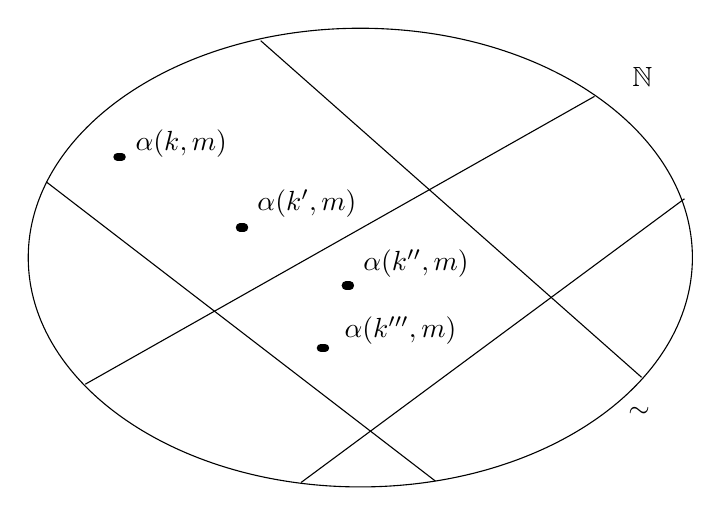
\begin{tikzpicture}[x=0.75pt,y=0.75pt,yscale=-1,xscale=1]
	%uncomment if require: \path (0,739); %set diagram left start at 0, and has height of 739
	
	%Shape: Ellipse [id:dp9650618878961996] 
	\draw   (23.5,124.5) .. controls (23.5,63.47) and (95.13,14) .. (183.5,14) .. controls (271.87,14) and (343.5,63.47) .. (343.5,124.5) .. controls (343.5,185.53) and (271.87,235) .. (183.5,235) .. controls (95.13,235) and (23.5,185.53) .. (23.5,124.5) -- cycle ;
	%Straight Lines [id:da5240208167193734] 
	\draw    (135.5,20) -- (319,182.17) ;
	%Straight Lines [id:da29391365058759567] 
	\draw    (32.17,88) -- (219.67,232.17) ;
	%Straight Lines [id:da8926403422381457] 
	\draw    (51,185.5) -- (296.33,46.83) ;
	%Straight Lines [id:da020284257694958674] 
	\draw    (155,232.83) -- (339.67,96.17) ;
	%Shape: Free Drawing [id:dp14447012165158735] 
	\draw  [color={rgb, 255:red, 0; green, 0; blue, 0 }  ][line width=3] [line join = round][line cap = round] (66.5,76) .. controls (67.17,76) and (67.83,76) .. (68.5,76) ;
	%Shape: Free Drawing [id:dp8018216878137716] 
	\draw  [color={rgb, 255:red, 0; green, 0; blue, 0 }  ][line width=3] [line join = round][line cap = round] (125.5,110) .. controls (126.17,110) and (126.83,110) .. (127.5,110) ;
	%Shape: Free Drawing [id:dp5726072331827443] 
	\draw  [color={rgb, 255:red, 0; green, 0; blue, 0 }  ][line width=3] [line join = round][line cap = round] (176.5,138) .. controls (177.17,138) and (177.83,138) .. (178.5,138) ;
	%Shape: Free Drawing [id:dp6843798478967522] 
	\draw  [color={rgb, 255:red, 0; green, 0; blue, 0 }  ][line width=3] [line join = round][line cap = round] (164.5,168) .. controls (165.17,168) and (165.83,168) .. (166.5,168) ;
	
	% Text Node
	\draw (74,61.73) node [anchor=north west][inner sep=0.75pt]    {$\alpha ( k,m)$};
	% Text Node
	\draw (132.67,90.4) node [anchor=north west][inner sep=0.75pt]    {$\alpha ( k',m)$};
	% Text Node
	\draw (313.33,31.73) node [anchor=north west][inner sep=0.75pt]    {$\mathbb{N}$};
	% Text Node
	\draw (311.33,195.4) node [anchor=north west][inner sep=0.75pt]    {$\sim $};
	% Text Node
	\draw (183.67,119.57) node [anchor=north west][inner sep=0.75pt]    {$\alpha ( k'',m)$};
	% Text Node
	\draw (174.67,151.57) node [anchor=north west][inner sep=0.75pt]    {$\alpha ( k''',m)$};
	\end{tikzpicture}
\end{center}
Dove il numero di classi di equivalenza è limitato dal numero di classi di equivalenza di $\sim$, e sappiamo che $\sim$ ha un numero finito di classi di equivalenza, quindi anche $\congAlpha$ avrà un numero finito di classi di equivalenza.



\subsection*{Esercizio 2.44}
\textit{Dimostrare la chiusura della classe dei linguaggi riconosciuti dagli automi di \buchi deterministici rispetto alle operazioni di unione e intersezione}

Siano $\mathcal{A} = (\mathcal{Q_A},A,\Delta_A,q_{0A},F_A)$ e $\mathcal{B} = (\mathcal{Q_B},A,\Delta_B,q_{0B},F_B)$

\textbf{Unione}: Se assumiamo che $ \mathcal{Q_A} \cap \mathcal{Q_B} = \emptyset$ allora possiamo costruire l'automa unione $\mathcal{C}$ come segue:
\begin{itemize}
	\item $\mathcal{Q_C} = \mathcal{Q_A} \cup \mathcal{Q_B} \cup \{q_{0C}\}$
	\item $A$ rimane invariato
	\item $\Delta_C = \Delta_A \cup \Delta_B$
	\item $q_{0C}$ come nuovo stato iniziale, con le stesse relazioni di $q_{0A}$ e $q_{0B}$, finale nel caso che almeno uno tra $q_{0A}$ e $q_{0B}$ sia uno stato finale
	\item $F_C = F_A \cup F_B$
\end{itemize}
\textbf{Intersezione}: Costruiamo l'automa intersezione $\mathcal{C}$, partendo dal prodotto cartesiano degli stati:
\begin{itemize}
	\item $\mathcal{Q_C} = \mathcal{Q_A} \times \mathcal{Q_B} \times \{1,2\}$
	\item $A$ rimane invariato
	\item $\Delta_C = \Delta_1 \cup \Delta_2$ dove
	\begin{itemize}
		\item $\Delta_1 = \{ ((q_A,q_B,1),a,(q_{A}',q_{B}',i)) \; | \; (q_A,a,q_A') \in \Delta_A\;e\;(q_B,a,q_B') \in \Delta_B\;e\;se\;q_A\in F_A\;allora\;i=2\;altrimenti\;i=1\}$
		\item $\Delta_2 = \{ ((q_A,q_B,2),a,(q_{A}',q_{B}',i)) \; | \; (q_A,a,q_A') \in \Delta_A\;e\;(q_B,a,q_B') \in \Delta_B\;e\;se\;q_B\in F_B\;allora\;i=1\;altrimenti\;i=2\}$
	\end{itemize}
	\item $q_{0C} = (q_{0A},q_{0B},1)$
	\item $F_C = \{(q_a,q_b,2)\;|\;q_B \in F_B\}$
\end{itemize}
Per costruzione, $r_C=(q_{A}^0,q_{B}^0,i^0),(q_{A}^1,q_{B}^1,i^1),\ldots$ è un'esecuzione su $\mathcal{C}$ per la parola w se:
\begin{itemize}
	\item $r_A=q_{A}^0,q_{A}^1,\ldots$ è un'esecuzione su $\mathcal{A}$ per w
	\item $r_B=q_{B}^0,q_{B}^1,\ldots$ è un'esecuzione su $\mathcal{B}$ per w
\end{itemize}
$r_A$ e $r_B$ sono accettate se $r_C$ è la concatenazione di una serie infinita di segmenti finiti di stati 1 (stati con terza componente 1) e stati 2 (stati con terza componente 2) alternativamente. Questa sequenza esiste se $r_C$ è accettato da $\mathcal{A}$ 
\subsection*{Esercizio 2.46}
\textit{Sia $A=\{a,b\}$ e $L=\{\alpha \in A^\omega. \exists^{<\omega}\;n\;\alpha(n)=a\}$. Si costruisca un automa di \buchi non deterministico che riconosca il linguaggio $L$}
 
\begin{center}
\begin{tikzpicture}[shorten >=1pt,node distance=2cm,on grid,auto] 
   \node[state,initial] (q_0)   {$q_0$};  
   \node[state,accepting] (q_1) [right=of q_1] {$q_1$};
    \path[->] 
    (q_0) edge [loop above] node {a,b} (q_0)
          edge node {a,b} (q_1)
    (q_1) edge [loop above] node  {b} (q_1);
\end{tikzpicture}
\end{center}


\subsection*{Esercizio 2.48}
\textit{Sia $A=\{a,b\}$ e $L=\overrightarrow{\{b^*a^*\}}$. Si costruisca un automa di \buchi non deterministico che riconosca il linguaggio $L$}

\begin{center}
\begin{tikzpicture}[shorten >=1pt,node distance=2cm,on grid,auto] 
   \node[state,initial,accepting] (q_0)   {$q_0$};  
   \node[state,accepting] (q_1) [right=of q_1] {$q_1$};
    \path[->] 
    (q_0) edge [loop above] node {b} (q_0)
          edge node {a,b} (q_1)
    (q_1) edge [loop above] node  {a} (q_1);
\end{tikzpicture}
\end{center}


\subsection*{Esercizio 2.50}
\textit{Dimostrare che la classe degli $\omega$-linguaggi $\omega$-regolari coincide con la classe degli $\omega$-linguaggi riconosciuti dagli automi di Muller non deterministici}

Dato che un $\omega$-linguaggio per essere $\omega$-regolare deve essere accettato da un automa di \buchi, mi basta dimostrare l'equivalenza tra gli automi di \buchi non deterministici e quelli di Muller non deterministici.

Sia $\Buchi$ un automa di \buchi, possiamo costruire un automa di Muller: $\mathcal{M} = (\mathcal{Q},A,\Delta,q_0,\mathcal{F})$ dove $\mathcal{F} = \{ X | X \in 2^Q \land X \cap F \neq \emptyset\}$. Si può osservare che una $\omega$-parola viene accettata da $\A$ se e solo se passa infinite volte per uno stato finale. Quindi viene accettata anche da $\mathcal{M}$ perchè, presa una sua computazione $\sigma$, abbiamo che $In(\sigma) \cap F \neq \emptyset $ e $ In(\sigma) \in 2^Q \Rightarrow In(\sigma) \in \mathcal{F}$ quindi la stessa $\omega$-parola viene accettata da $\mathcal{F}$. Lo stesso ragionamento lo possiamo fare al contrario. Se una $\omega$-parola viene accettata da $\mathcal{M}$ allora $In(\sigma) \cap F \neq \emptyset $ quindi esiste una computazione che passa infinite volte per uno stato finale, quindi 
la stessa $\omega$-parola viene accettata da $\A$. 

\subsection*{Esercizio 2.57}
\textit{Dimostrare che l'insieme $W_V\subseteq A^*$ dei V-testimoni, con V classe di congruenza $\approx_\mathcal{A}$ è regolare}

Ri


\section{Exercices of chapter 0 of Temporal Verification of Reactive Systems}

\section{Additional exercices}
\subsection*{Esercizio1}
\textit{Dato un linguaggio $L \subseteq A^*$, dimostrare se che $L$ è un linguaggio star-free, allora $L$ è definibile nel frammento al prim'ordine di $S1S_A$, con la relazione di ordinamento $<$ e i predicati unari $Q_a$, con $a \in A$.}


\subsection*{Esercizio2}
\textit{Dimostrare che l'insieme dei linguaggi riconosciuti da automi di \buchi su alberi infiniti con insieme degli stati finali singoletto è strettamente contenuto nell'insieme dei linguaggi riconosciuti da automi di \buchi su alberi infiniti}


\subsection*{Esercizio3}
\textit{Sia $A=\{a,b\}$ e $T_1=\{t\in T^{\omega}_A:$tutti i cammini di t contengono un numero finito di occorrenze di a$\}$. $T_1$ contiene l'insieme di tutti gli alberi $t_i$, con $i\geqslant 0$, tali che $t_i$ ha un'occorrenza di a nelle posizioni $\epsilon, 1^{m_1}0,\ldots,1^{m_1}01^{m_2}0\ldots 1^{m_i}0$, con $m_1,m_2,\ldots,m_i>0$. Immaginiamo che esista un automa di \buchi $\Buchi$ con $n+1$ stati, con $n\geqslant 1$, incluso lo stato iniziale $q_0$ che occorre solo in posizione $\epsilon$ tale che $L(\A)=T_1$ e sia r un run di successo di $\A$ su $t_n$. Mostrare che deve esistere un cammino in $t_n$ contenente 3 nodi u,v e w, con $u<v<w$, tali che $r(u)=r(w)=s \in F e t_n(v)=a$.}


\subsection*{Esercizio4}
\textit{Siano $C=\{c_1,\ldots,c_m\}$ e \=c$= ( c_1,\ldots,c_m) $. Sia dato $T \subseteq T^{\omega}_A$ tale che $T=T_0 \cdot$\=c$(T_1,\ldots,T_m)^{\omega}$}


\subsection*{Esercizio5}
\textit{Dimostrare la (correttezza e completezza della) caratterizzazione di uno degli operatori di CTL (diverso da AF) quale minimo punto fisso di un’opportuna trasformazione di predicato.}


\subsection*{Esercizio6}
\textit{Dimostrare la (correttezza e completezza della) caratterizzazione di uno degli operatori di CTL (diverso da EG) quale massimo punto fisso di un’opportuna trasformazione di predicato.}



\end{document}
